空間データにおけるSelf-Attention機構とは、ある点の値をその周りすべての点の加重和で
表現するための機構となっている。従来の畳み込み処理でも似たような処理が行われるが、すべての点
ではなく一定領域の点のみが畳み込みに用いたられる。したがって空間全体の情報を取り込むことがで
きなかった。しかしSelf-Attention機構では対象データ点を除く空間内すべてのデータ点の情報を取り
込むことでより空間全体の特徴を捉えることが可能になった。

Self-Attention機構は空間全体との関連度合いを計算して、入力データを重みづけして出力する処理を行っている。
したがって入力と出力の形式は同じ変換処理となる。計算の概要図を\ref{fig:self-attention-memory-module}左側に示す。

\begin{figure}[H]
\begin{center}
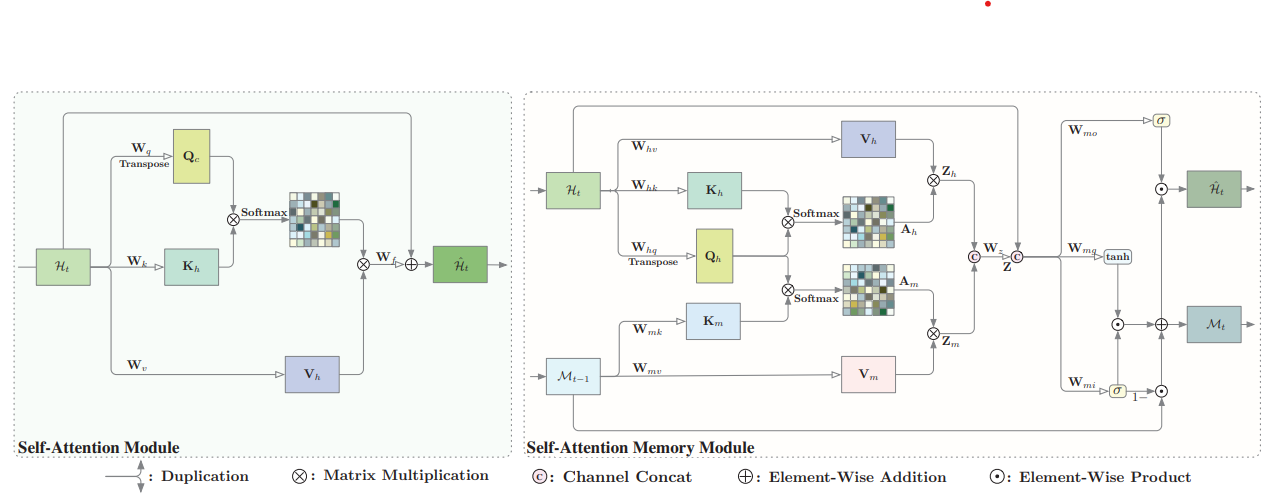
\includegraphics[width=\linewidth]{fig/methodologies/self-attention-memory-module.png}
\captionsetup{width=0.9\linewidth}
\caption{Lin \textit{et al}.[2020] Figure1より引用。Self-Attention機構の計算概要図(左側)とSelf-Attentionメモリー機構の計算概要図(右側)。}
\label{fig:self-attention-memory-module}
\end{center}
\end{figure}

Self-Attention機構では入力$\mathcal{H}_{t}$に対して以下の3つの特徴空間が計算される。

\begin{align}
	\boldsymbol{query:} \boldsymbol{Q}_{h} &= \boldsymbol{W}_{q}\mathcal{H}_{t} \in \mathbb{R}^{\hat{C} \times N} \\
	\boldsymbol{key:} \boldsymbol{K}_{h} &= \boldsymbol{W}_{k}\mathcal{H}_{t} \in \mathbb{R}^{\hat{C} \times N} \\
	\boldsymbol{value:} \boldsymbol{V}_{v} &= \boldsymbol{W}_{v}\mathcal{H}_{t} \in \mathbb{R}^{C \times N}
\end{align}

% textlint-disable
$\boldsymbol{W}_{q}$、$\boldsymbol{W}_{q}$、$\boldsymbol{W}_{q}$は入力$\mathcal{{H}_{t}}$の
全データ点における$\boldsymbol{query}$、$\boldsymbol{key}$、$\boldsymbol{value}$の重みである。
また$C$と$\hat{C}$は入力データのチャンネル数である。$N$は入力データの総データ点数($H \times W$)で
ある。Self-Attention機構ではあるデータ点同士の類似度$\boldsymbol{e}$が以下のように計算される。
% textlint-enable

\begin{equation}
\boldsymbol{e} = \boldsymbol{Q}_{h}^T\boldsymbol{K}_{h} \in \mathbb{R}^{N \times N}
\end{equation}

したがって$i$番目のデータ点と$j$番目のデータ点との関連度は$e_{i,j} = (\mathcal{H}_{t,i}^T\boldsymbol{W}_{q}^T)(\boldsymbol{W}_{k}\mathcal{H}_{t,j})$
となる。$\mathcal{H}_{t,j}$と$\mathcal{H}_{t,j}$はそれぞれ$i$番目と$j$番目のチャンネルに対応したベクトルである。
さらに以下のように正規化することで最終的な関連度が得られる。

\begin{equation}
\alpha_{i,j} = \frac{\exp(e_{i,j})}{\sum_{k=1}^{N}\exp(e_{i,k})}, i,j \in {1, 2, ..., N}.
\end{equation}

$i$番目のデータ点におけるSelf-Attention機構の最終的な出力は以下のように表される。

\begin{equation}
\boldsymbol{Z}_{i} = \sum_{j=1}^N\alpha_{i,j}(\boldsymbol{W}_{v}\mathcal{H}_{t;j})
\end{equation}

$\boldsymbol{W}_{v}\mathcal{H}_{t;j} \in \mathbb{R}^{C \times 1}$は$\boldsymbol{value: V_{h}}$の
$j$番目のチャンネルに対応したベクトルである。最終的に$i$番目のデータが空間全体のデータ点に対する
関連度合いで重みづけされて変換されていることがわかる。